\documentclass[aps,pra,twocolumn,10pt]{revtex4-1}
\usepackage{amssymb}
\usepackage{amsfonts}
\usepackage[fleqn,tbtags]{amsmath}
\usepackage{graphicx} 


\begin{document}

\title{Quantum Annealing for Air Traffic Management}
\author{Tobias Stollenwerk}
\affiliation{German Aerospace Center, Linder H\"ohe, 51147 Cologne, Germany}
\author{Bryan O'Gorman},
\author{Salvatore Mandr\`{a}}
\author{Eleanor G. Rieffel}
%\author{Davide Venturelli},
%\author{Olga Rodionova},
%\author{Hok K. Ng},
%\author{Banavar Sridhar},
\affiliation{NASA Ames, Moffet Blvd, Mountain View, CA 94035, USA}
\date{\today}

\maketitle


%%%%%%%%%%%%%%%%%%%%%%%%%%%%%%%%%%%%%%%%%%%%%%%%%%%%%%%%%%%%%%%%%%%%%%%%%%%%%%
%%%%%%%%%%%%%%%%%%%%%%%%%%%%%%%%%%%%%%%%%%%%%%%%%%%%%%%%%%%%%%%%%%%%%%%%%%%%%%
%%%%%%%%%%%%%%%%%%%%%%%%%%%%%%%%%%%%%%%%%%%%%%%%%%%%%%%%%%%%%%%%%%%%%%%%%%%%%%
%%%%%%%%%%%%%%%%%%%%%%%%%%%%%%%%%%%%%%%%%%%%%%%%%%%%%%%%%%%%%%%%%%%%%%%%%%%%%%
%%%%%%%%%%%%%%%%%%%%%%%%%%%%%%%%%%%%%%%%%%%%%%%%%%%%%%%%%%%%%%%%%%%%%%%%%%%%%%
\section{Introduction}


%%%%%%%%%%%%%%%%%%%%%%%%%%%%%%%%%%%%%%%%%%%%%%%%%%%%%%%%%%%%%%%%%%%%%%%%%%%%%%
%%%%%%%%%%%%%%%%%%%%%%%%%%%%%%%%%%%%%%%%%%%%%%%%%%%%%%%%%%%%%%%%%%%%%%%%%%%%%%
%%%%%%%%%%%%%%%%%%%%%%%%%%%%%%%%%%%%%%%%%%%%%%%%%%%%%%%%%%%%%%%%%%%%%%%%%%%%%%
%%%%%%%%%%%%%%%%%%%%%%%%%%%%%%%%%%%%%%%%%%%%%%%%%%%%%%%%%%%%%%%%%%%%%%%%%%%%%%
%%%%%%%%%%%%%%%%%%%%%%%%%%%%%%%%%%%%%%%%%%%%%%%%%%%%%%%%%%%%%%%%%%%%%%%%%%%%%%
\section{Problem Description}
The problem at hand is the deconflicting of transatlantic wind-optimal trajectories.
As it was done in \cite{rodionova16} we are using the same wind-optimal trajectories of a single day, July 29 2012.
These wind-optimal trajectories are given as
${\left(\mathbf{x}_i\right)}_{i=1}^n$, 
where 
$\mathbf{x}_i = {\left(x_{i,t}\right)}_{t=t_{i,0}}^{t_{i,1}}$ 
and 
$x_{i, t}$ is the location (as latitude, longitude, and altitude) of the $i$th flight at time $t$.
The times $t_{i,0}$ and $t_{i, 1}$ are the times at which the wind-optimal trajectory for the $i$th flight begins and ends, respectively.
Furthermore, the times are given in units of one minutes $T_i = \left(t_{i, 0}, t_{i, 0} + 1, \ldots, t_{i, 1}\right)$.
Each flight $i$ is at a constant speed $v_i$, to within (classical) machine precision.

A conflict between two flights is defined as a pair of trajectory points which are too close to each other in space and time.
\begin{equation} \label{eqn:conflicting_trajectory_points}
    \{ (x_{i, t},  x_{j, t'}) \; | \; \mathcal{D} (x_{i, t}, x_{j, t'}) < \Delta_x ,  |t - t'| < \Delta_t \} \; ,
\end{equation}
where $\mathcal{D}(x, y)$ is the spatial distance between two points $x$ and $y$ given as latitude, longitude and altitude.
Following \cite{rodionova16}, the space threshold is $\Delta_x = 3$ nautical miles and the time threshold is $\Delta_t = 3$ minutes.
In this paper, we consider the following means to deconflict the trajectories:
First, we can delay each flight $i$ at departure time by a departure delay $d_i$
\begin{equation*}
    x_{i, t} \to x_{i, t + d_i} \quad \forall \; t \in T_{i}
\end{equation*}

Second, we can avoid a conflict by maneuvers of both involved flights.
We assume, however, that the maneuvers will not introduce new conflicts. 
In doing so, these maneuvers can be view as resulting in time shifts only.

%%%%%%%%%%%%%%%%%%%%%%%%%%%%%%%%%%%%%%%%%%%%%%%%%%%%%%%%%%%%%%%%%%%%%%%%%%%%%%
%%%%%%%%%%%%%%%%%%%%%%%%%%%%%%%%%%%%%%%%%%%%%%%%%%%%%%%%%%%%%%%%%%%%%%%%%%%%%%
%%%%%%%%%%%%%%%%%%%%%%%%%%%%%%%%%%%%%%%%%%%%%%%%%%%%%%%%%%%%%%%%%%%%%%%%%%%%%%
\subsection{Classical Preprocessing}
It is beneficial to reduce the data to conflicting regions in space and decoupling the spacial and temporal components of the problem.
As a first step, we detect all pairs of trajectory points which are separated by a spacial distance below $\Delta_x$ 
\begin{equation*}
    \{ (x_{i, t},  x_{j, t'}) \; | \; \mathcal{D} (x_{i, t}, x_{j, t'}) < \Delta_x \} \; ,
\end{equation*}
Two spatially conflicting trajectory points might never become conflicting in time if the corresponding times are far apart.
By introducing a constant maximum delay $D_{max}$ we can dismiss all spatial conflicts which can never become conflicting in time
\begin{equation*}
    \{ (x_{i, t},  x_{j, t'}) \; | \; \mathcal{D} (x_{i, t}, x_{j, t'}) < \Delta_x , |t-t'| \geq \Delta_t + D_\text{max} \} \; .
\end{equation*}
With this, we are left with a set of potentially conflicting pairs of trajectory points
\begin{equation*}
    C^{ij}_0 = \{ (x_{i, t},  x_{j, t'}) \; | \; \mathcal{D} (x_{i, t}, x_{j, t'}) < \Delta_x , |t-t'| < \Delta_t + D_\text{max} \} \; .
\end{equation*}

As a next step, we group together conflicting trajectory point pairs which are subsequent in time
\begin{align*}
    C^{ij}_\parallel = \{ ((x_{i, t},  x_{j, t'}),  (x_{i, s},  x_{j, s'})) \; | \; & (x_{i, t},  x_{j, t'}) \in C^{ij}_0, \\
                                                                                    & (x_{i, s},  x_{j, s'}) \in C^{ij}_0, \\ 
                                                                                    & |t - s| < \Delta'_t,  \\
                                                                                    & |t' - s'| < \Delta'_t \}
\end{align*}
where we set $\Delta'_t = 2$ minutes.

\begin{figure}[t]
    \begin{center}
        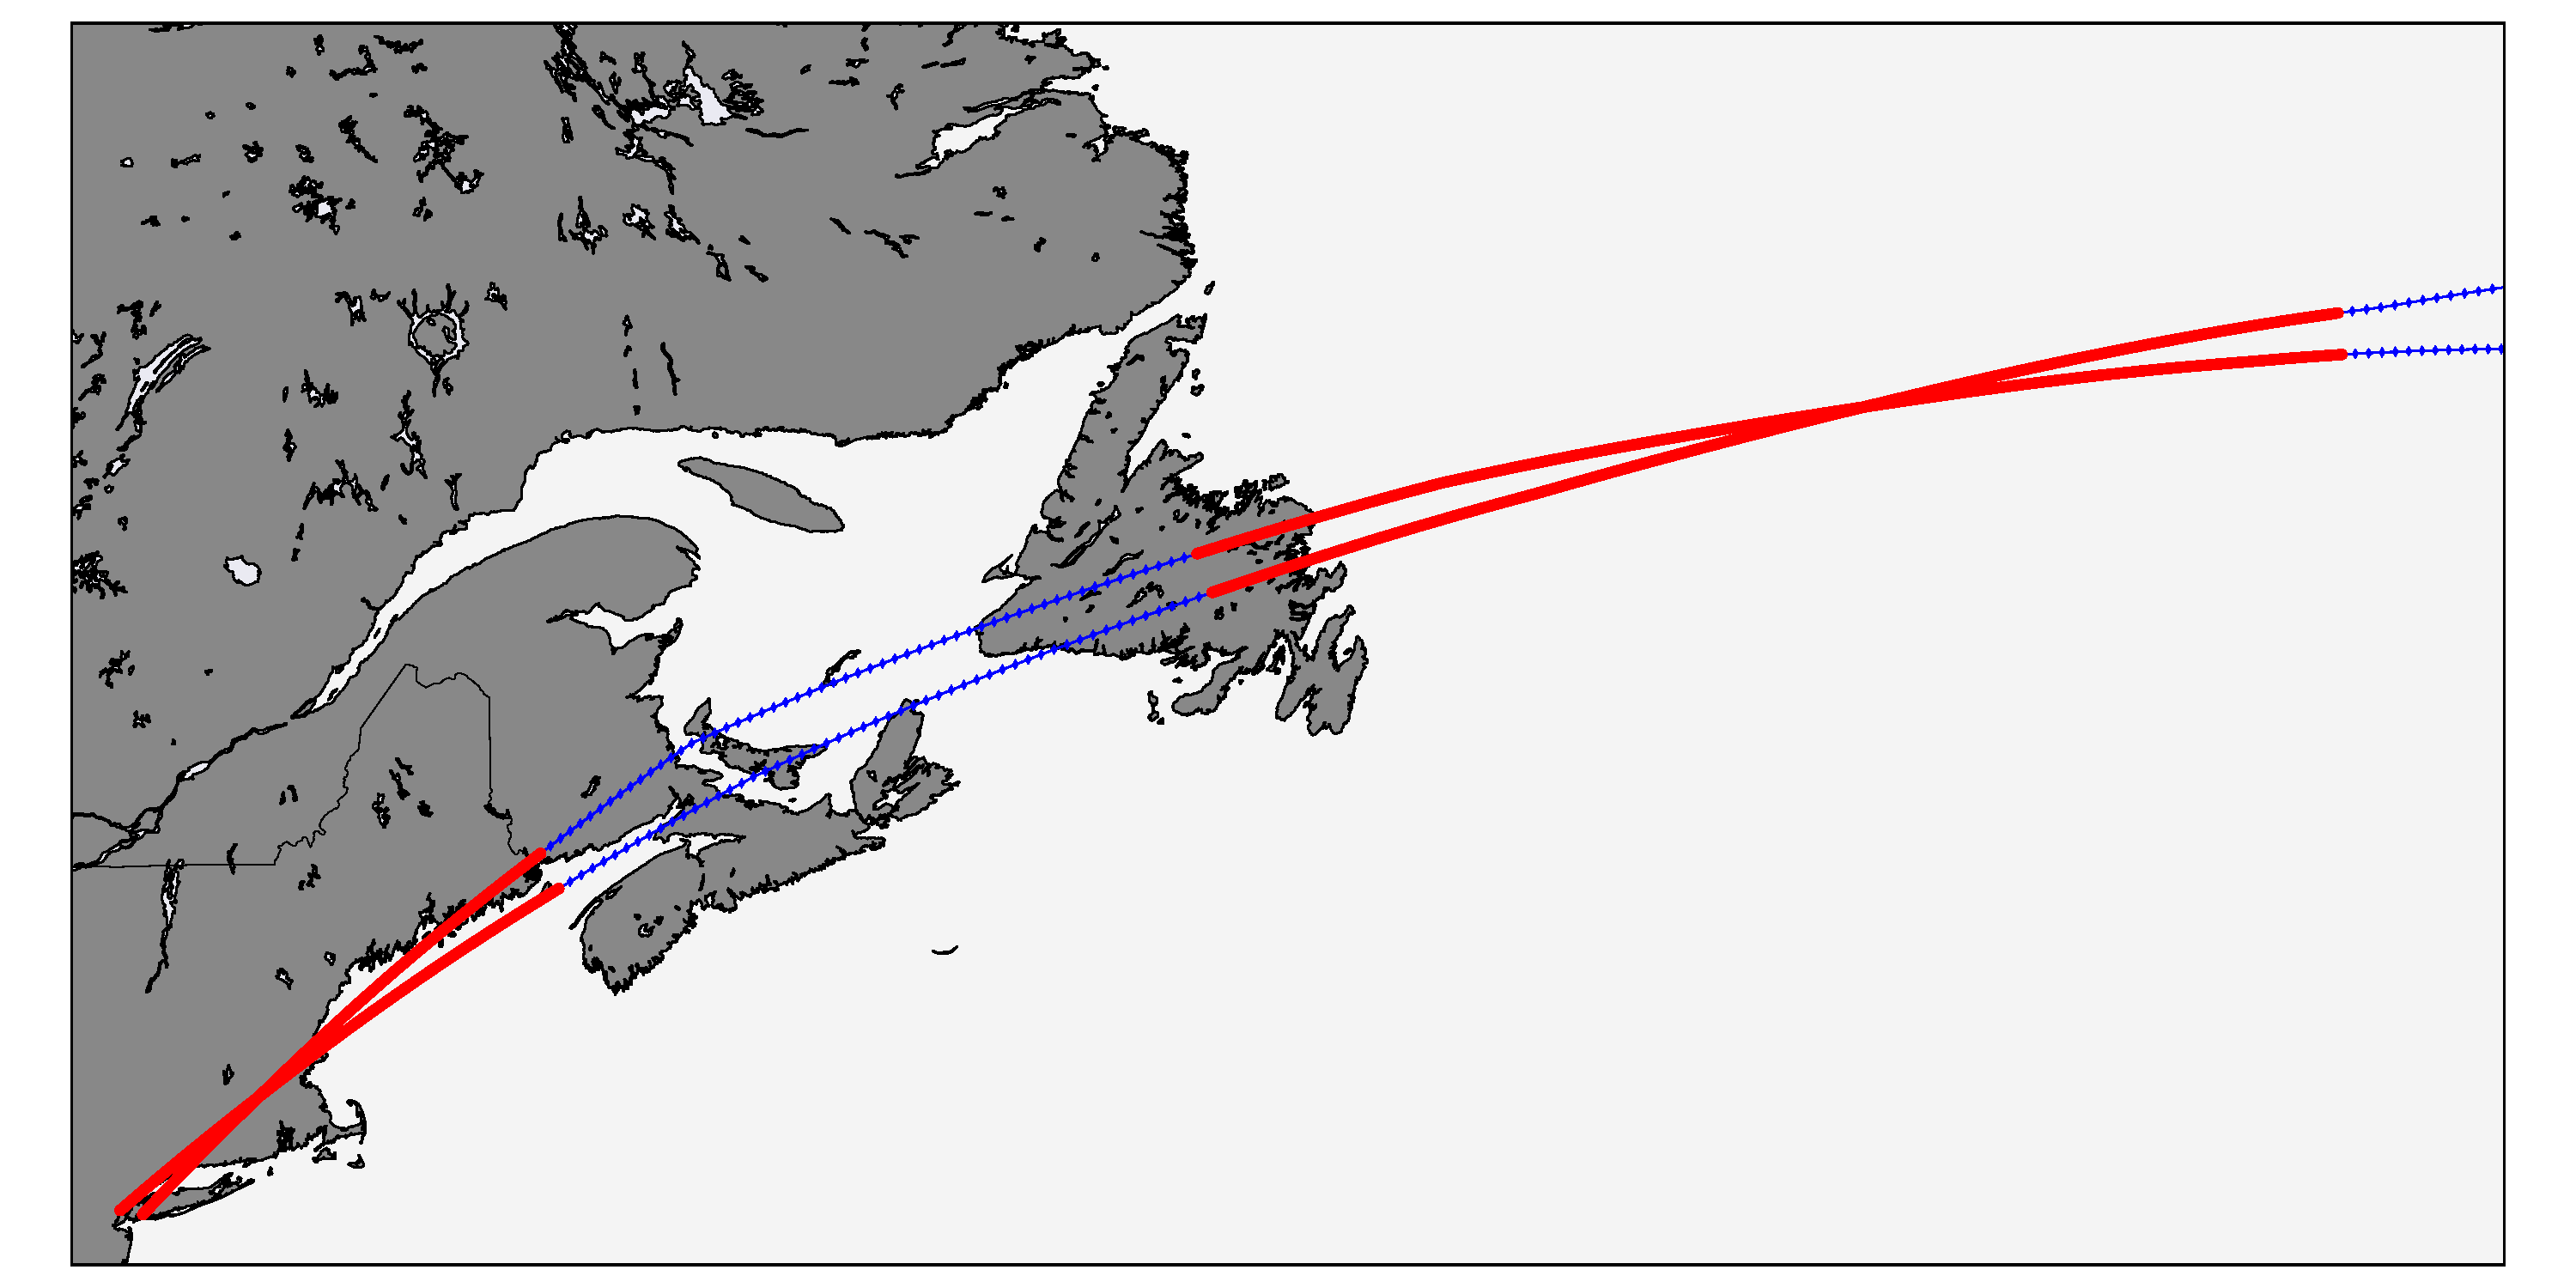
\includegraphics[width=0.45\textwidth,natwidth=1,natheight=0]{./pics/example_conflict_in_real_space.pdf}
    \end{center}
    \caption{Example of two parallel potential conflicts between two transatlantic flights starting from the east cost of the USA.}
    \label{fig:example_parallel_conflict}
\end{figure}

For a given pair of flights $(i, j)$ there might be multiple ``disjoint`` subsets in $C^{ij}_\parallel$
\begin{equation*}
    \bigcup_{n} C^{ij}_{\parallel n} = C^{ij}_\parallel
\end{equation*}
where
\begin{align*}
    & |t - s| \geq \Delta'_t \land |t' - s'| \geq \Delta'_t \\
    & \forall (x_{i, t},  x_{j, t'}) \in C^{ij}_{\parallel n}, \\
    & \forall (x_{i, s},  x_{j, s'}) \in C^{ij}_{\parallel n'}, \\
    & n \neq n' \; .
\end{align*}
In figure \ref{fig:example_parallel_conflict} an example of two separated clusters are shown.
Together with the remaining, spatially isolated, conflicting trajectory points
\begin{equation*}
    C^{ij}_{\times} = C^{ij}_0 \setminus C^{ij}_\parallel \; ,
\end{equation*}
these subsets of trajectory point clusters are called \emph{potential conflicts}.
\begin{equation*}
    C_k \in C = \{ C^{ij}_{\parallel n} | \forall i, j, n\} \cup  \{C^{ij}_{\times} | \forall i, j\}
\end{equation*}
Here, we introduced a conflict index $k\in\{1, \dots, N_C\}$, with $N_C = |C|$.
For each conflict index $k$, we will denote the pair of involved flights by $I_k = (i_k, j_k)$.

\begin{figure}[t]
    \begin{center}
        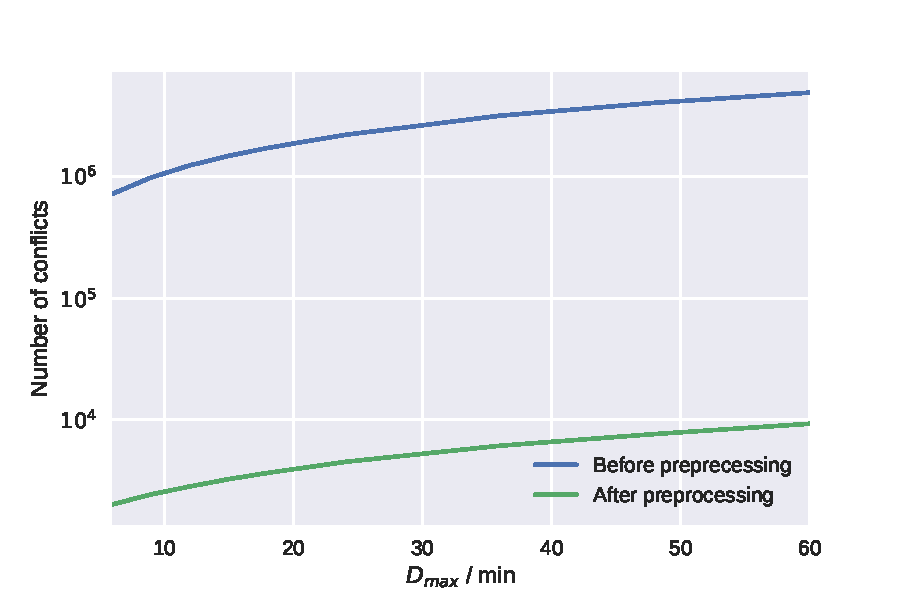
\includegraphics[width=0.45\textwidth,natwidth=1,natheight=0]{./pics/preprocessing_reduction_number_of_conflicts.pdf}
    \end{center}
    \caption{Preprocessing: Reduction in the number of potential conflicts for various upper delay bounds $D_\text{max}$.}
    \label{fig:preprocessing_reduction_number_of_conflicts}
\end{figure}

Before the preprocessing, the number of conflicts was given by $N_C^\text{before} = \sum_{ij} |C^{ij}_0|$.
As one can see in figure \ref{fig:preprocessing_reduction_number_of_conflicts} the preprocessing reduces the number of conflicts by orders of magnitude.

%%%%%%%%%%%%%%%%%%%%%%%%%%%%%%%%%%%%%%%%%%%%%%%%%%%%%%%%%%%%%%%%%%%%%%%%%%%%%%
%%%%%%%%%%%%%%%%%%%%%%%%%%%%%%%%%%%%%%%%%%%%%%%%%%%%%%%%%%%%%%%%%%%%%%%%%%%%%%
%%%%%%%%%%%%%%%%%%%%%%%%%%%%%%%%%%%%%%%%%%%%%%%%%%%%%%%%%%%%%%%%%%%%%%%%%%%%%%
\subsection{Conflict Avoidance}
In order to avoid conflicts, a flight $i$ can be either delayed at departure time by $d_i$ or by maneuver introduced delays $d_{ik}$ for each conflict $k$ the flight is involved in.
With this, the trajectory times of flight $i$ are shifted
\begin{align*}
    t_i & \to \tau_i = t_i  + D_i(t) \; , \\
    D_i(t) & = d_i + \sum_{k\in K_{i}(t)} d_{ik} 
\end{align*}
where $D_i(t)$ is the delay of flight $i$ at time $t$ and the sum runs over all the conflicts which are before $t$
\begin{equation*}
    K_{i}(t) = \{k | \max_{t'} x_{i,t'} \in C_k < t   \} 
\end{equation*}
We introduce the pairs of times of spatially conflicting points inside a conflict $k$:
\begin{equation*}
    T_k =  \{(t, t') \; | \; |x_{i, t} - x_{j, t'}| < \Delta_x, (i, j) \in I_k \}
\end{equation*}
A conflicts $k$ between two flights $i$ and $j$ occurs if the delays are chosen such that a temporal difference between spatially conflicting points is below $\Delta_t$:
\begin{align*}
    & |t + D_i(t) - t' - D_j(t')| < \Delta_t \\
    \Rightarrow  & - \Delta_t - (t - t') < D_i(t) - D_j(t') < \Delta_t - (t - t')
\end{align*}
for any $(t, t') \in T_k$.
Hence a conflict $k$ is avoided if
\begin{equation*}
    D_i(t) - D_j(t') \notin D_k
\end{equation*}
with
\begin{equation*}
    D_k = \left(-\Delta_t - \max_{(t, t') \in T_k} (t - t'), \Delta_t - \min_{(t, t') \in T_k} (t - t')\right)
\end{equation*}
\section{Mapping to QUBO}


\bibliography{atm}

\end{document}
